\chapter{Grafisk løsning}
%
% 2.1 Polyeder og konvekse mængder 
% ---------------------------------------------------------
	\input{incl/main/grafisk_losning/hyperplan_halvrum_polyeder}
	\input{incl/main/grafisk_losning/konvekse_maengder}
% 
%
% 2.2 Ekstrema, hjørnepunkter og basale mulige løsninger 
% ---------------------------------------------------------
	\section{Ekstremer, hjørnepunkter og basale løsninger}
%
%\textit{Vis at løsningerne findes i hjørnene af en polytede.}
Som det fremgår af afsnit \ref{heeeeejjulle}, vil en optimal løsning være tilbøjelige til at ligge i hjørnerne af en polyede.
Der er derfor behov for måder at definere disse hjørner på.
%
\begin{defn}{}{ekstrema}
Lad $\mathcal{P}$ være en polyede. 
En vektor $\mathbf{x} \in \mathcal{P}$ kaldes et \textbf{ekstremumspunkt} i $\mathcal{P}$, hvis der ikke eksisterer to vektorer $\mathbf{y},\mathbf{z} \in \mathcal{P}$, $\mathbf{y} \land \mathbf{z} \neq \mathbf{x}$, 
samt en skalar $\lambda \in [0,1]$, hvorom det gælder: $\mathbf{x}=\lambda\mathbf{y}+(1-\lambda)\textbf{z}$.
\end{defn}
\noindent
%
%
Et hjørne kan beskrives ud fra denne definition idet der såfremt $\mathbf{x}=\lambda\mathbf{y}+(1-\lambda)z$, og alle vektorene findes i $P$, gælder at $\mathbf{x}$ er en konveks kombination af $\mathbf{y}$ og $\mathbf{z}$.
Hvis $\mathbf{x}=\lambda\mathbf{y}+(1-\lambda)\textbf{z}$ og $\mathbf{x}$ er et ekstremumspunkt må det derfor gælde at $\mathbf{y}\notin P$ eller $\mathbf{z}\notin P$ eller $\mathbf{x}=\mathbf{z}$ eller $\mathbf{x}=\mathbf{y}$. 
Det skal her nævnes at denne definition er strengt geometrisk.
%

\begin{figure}[h!]
  \centering
  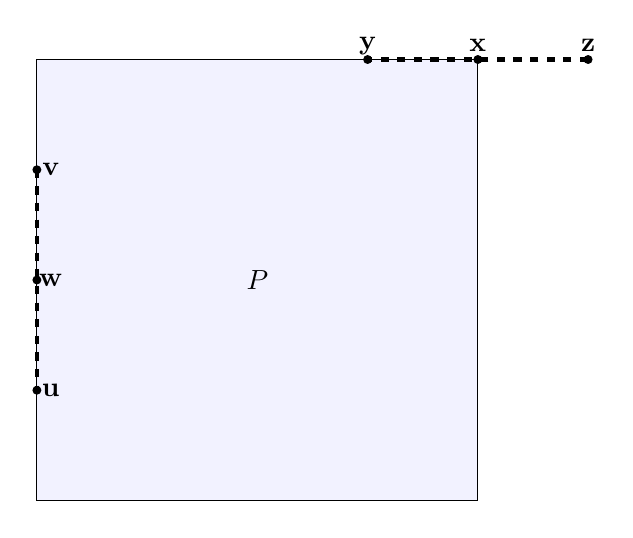
\begin{tikzpicture}[scale=0.7]
    \tikzset{punkt/.style={point, draw=black}}
    
    
%Punkter

	\node at (4,4)	(1){};
	\node at (-4,4)	(4){};
	\node at (4,-4)	(2){};
	\node at (-4,-4) (3){};


	\filldraw[black, fill=blue!5] (2) rectangle (4);
	\node at (0,0) (P){$P$};
	
	\filldraw [black] (2,4) circle (2pt);
	\filldraw [black] (4,4) circle (2pt);
	\filldraw [black] (6,4) circle (2pt);
	\filldraw [black] (-4,2) circle (2pt);
	\filldraw [black] (-4,0) circle (2pt);
	\filldraw [black] (-4,-2) circle (2pt);	
	\node at (2,4.25)	 (y){$\textbf{y}$};
	\node at (4,4.25)	 (x){$\textbf{x}$};
	\node at (6,4.25)	 (z){$\textbf{z}$};
	\node at (-3.75,2)  (v){$\textbf{v}$};
	\node at (-3.75,0)	 (w){$\textbf{w}$};
	\node at (-3.75,-2) (u){$\textbf{u}$};


	\draw[-, dashed,black,ultra thick] (6,4) -- (2,4);
	\draw[-, dashed,black,ultra thick] (-4,2) -- (-4,-2);

  \end{tikzpicture}
  \caption{En afgrænset polytop $P$ hvor $\textbf{x}$ er et ekstramapunkt da der ikke findes vektorer $\textbf{y}$ og $\textbf{z}$ sådan at $\mathbf{x}=\lambda\mathbf{y}+(1-\lambda)z$. $\textbf{w}$ er i modsætning ikke et ekstremapunkt da der findes $\textbf{v}$ og $\textbf{u}$ sådan at $\mathbf{w}=\lambda\mathbf{v}+(1-\lambda)u$.}
  \label{fig:ekstrema}
\end{figure}
%
%
%    \node[punkt] at (-4,0.5)      (v1){$v_1$};
%    \node[punkt] at (-2,0.5)      (v2){$v_2$};
%    \node[punkt] at (-4,-1.5)     (v3){$v_3$};
%    \node[punkt] at (-2,-1.5)     (v4){$v_4$};
%    \node at (-3,2)     (v){$K_{4}$};
%
%
%    \node[punkt] at (4.6,-0.2)      (k1){$v_3$};
%    \node[punkt] at (1.4,-0.2)      (k2){$v_2$};
%    \node[punkt] at (2,-2)     (k3){$v_4$};
%    \node[punkt] at (4,-2)     (k4){$v_5$};
%    \node[punkt] at (3,1)      (k5){$v_1$};
%    \node at (3,2)      (k){$K_{5}$};
%
%
%
%
%
%    \draw [-, thick, draw=black] (v1) -- (v2);
%    \draw [-, thick, draw=black] (v1) -- (v3);
%    \draw [-, thick, draw=black] (v1) -- (v4);
%    \draw [-, thick, draw=black] (v2) -- (v3);
%    \draw [-, thick, draw=black] (v2) -- (v4);
%    \draw [-, thick, draw=black] (v3) -- (v4);
\\\\
%
En alternativ geometrisk definition relatere sig til \textit{hjørne punkter}, som er den entydige optimale løsning til et givet lineært programmeringsproblem med den mulige løsningsmængde $\mathcal{P}$.
%
\begin{defn}{}{hjoerner}
Lad $P$ være en polyede. 
En vektor $\mathbf{x}\in P$ siges at være et \textbf{hjørne punkt}, hvis der esksiterer en vektor $\mathbf{c}$, hvorom det gælder at $\mathbf{c}^T\mathbf{x}<\mathbf{c}^T\mathbf{y}$ for alle $\mathbf{y}$, som opfylder $\mathbf{y} \in P$ samt $\mathbf{y}\neq\mathbf{x}$.
\end{defn}
\noindent
%
%
Dette kan ligeledes beskrives som at $\mathbf{x}$ er et hjørne i $P$ såfremt $P$ er på den ene side af et hyperplan der skærer $P$ i $\mathbf{x}$. 
Jævnfør definitionen har dette hyperplan ligningen $y \mid \mathbf{c}^T\mathbf{x}=\mathbf{c}^T\mathbf{y}.$	
	\begin{defn}{}{algh}
Hvis en vektor $\textbf{x}$ opfylder $\textbf{a}^T_i\textbf{x}= b_i$ for $i \in M_1, M_2 \text{ eller } M_3$, så siges den tilsvarende betingelse at være \textbf{bindende} ved $\textbf{x}$.
\end{defn}\noindent
%
Følgende sætning giver anledning til hvordan disse bindende betingelser kan føres i relation til løsninger af lineære optimeringsproblemer.
%
\begin{thm}{}{}

Lad $\textbf{x}$ være et element i $\R^n$ og lad $I=\{i|\textbf{a}^T_i\textbf{x}=b_i\}$ være en mængde af indexer på betingelser, der er bindende ved $\textbf{x}$.
Så er følgende udsagn ækvivalente.
%
\begin{enumerate}[label=(\alph*)]
\item Der eksisterer $n$ vektorer i mængden $\{\textbf{a}_i|i \in I \}$, som er lineært uafhængige.
\item Spannet af vektorerne $\textbf{a}_i$, for $i$ i $I$, dækker hele $\R^n$.
\item Ligningssystemet $\textbf{a}^T_i\textbf{x}= b_i$, for $i \in I$, har en entydig løsning.
\end{enumerate}
\end{thm}
%
\begin{proof}
Smukt bevis INC.
\end{proof}
% 
%
% 2.3 Polyede på standardform
% ---------------------------------------------------------
	\section{Polyeder på standardform}
\label{afsnit:fisk}
%
Som det bliver beskrevet i afsnit \ref{sec:standard} kan optimeringsproblemer opskrives på standardform.
Dette korosponderer med polyeder der ligeledes kan opskrives på standardform: 
$P=\{ \mathbf{x} \in \R^n \mid A\mathbf{x}=\mathbf{b},x \geq 0 \}$, hvor er $A$ er en $m \times n$ matrix.
$P$ bliver er her et \textbf{polyede på standardform}.
I de fleste tilfælde er det en fordel at antage at de $m$ rækker i $A$ er lineært uafhængige.
%I sætning \ref{something something} vil det endvidere blive vist at rækker der ikke er uafhængige kan udelukkes fra løsningen.
som det ses i (ref til basale mulige løsninger) skal der være $n$ aktive-begrænsninger i spil for at finde en basal mulig løsning.
såfremt $m \neq n$, skal der derfor vælges $n-m$ variable $x_i$ med henblik på, at sætte disse $x_i=0$, hvilket gør begrænsningerne $x_i \geq 0$ aktive.
ovenstående 53 i bogen har behov for andre læser så vi kan diskutere hvad det betyder.
Det er dog ikke uvæsentligt hvilke af disse variable der omdannes til $0$ hvilket belyses af sætning \ref{thm:polystd}.
\begin{thm}{}{polystd}
Ved begrænsningerne $A\mathbf{x}=\mathbf{b}$ og $\mathbf{x}\geq 0$.
Antag at $A$ er en $m \times n$ og har lineært uafhængige rækker.
$\mathbf{x} \in \R^n$ er en basal løsning hvis og kun hvis: $A\mathbf{x}=\mathbf{b}$ og der eksisterer indexer $B(1),\ldots,B(m)$ hvorom det gælder:
\begin{enumerate}[label=(\alph*)]
\item Søjlerne $\mathbf{A}_{B(1)},\ldots,\mathbf{A}_{B(m)}$ er lineært uafhængige.
\item Hvis $i \neq \mathbf{A}_{B(1)},\ldots,\mathbf{A}_{B(m)}$, så er $x_i=0$.
\end{enumerate}
\end{thm}
\begin{proof}
Betragt et $x \in \R^n$ og antag at der eksiterer indexer $\mathbf{A}_{B(1)},\ldots,\mathbf{A}_{B(m)}$ der opfylder (a) og (b).
Da gælder om de aktive begrænsninger at $x_i=0$, når $i\neq B(1),\ldots,B(m)$, samt at $A\mathbf{x}=\mathbf{b}$.
Dette implicere, da liniært afhængige løsninger sættes lig $0$,  at 
$$\sum_{i=1}^{m}\textbf{A}_{B(i)}x_{B(i)}=\sum_{i=1}^{n}\textbf{A}_ix_i=A\textbf{x}=\textbf{b}$$.
Da søjlerne $\textbf{A}_{B(i)}x_{B(i)}$ for $i=1,\ldots,m$ er lineært uafhængige, kan $x_{B(1)},\ldots,x_{B(m)}$ bestemmes entydigt. 
Altså har ligningssystemet skabt af de aktive begrænsninger en entydig løsning.
Fra sætning (MAAADS), følger at der er $n$ aktive begrænsninger, hvorfor $\mathbf{x}$ er en basal løsning. 
Antag nu at $\mathbf{x}$ er en basal løsning, det skal nu vises at (a) og (b) da er opfyldt.
Lad $x_{B_1},\ldots,x_{B_k}$ være ikke-nul komponenter i $\textbf{x}$.
Da $\mathbf{x}$ er en basal løsning, følger nu at ligningssysemet givet ved de aktive begrænsninger $x_i=0$, når $i\neq B(1),\ldots,B(k)$, samt  $\sum_{i=1}^{n}\mathbf{A}_ix_i=\mathbf{b}$, har en entydig løsning. 
Det samme må derfor gøre sig gældende for $\sum_{i=1}^{k}\mathbf{A}_{B(i)}x_{B(i)}=\mathbf{b}$.
Det følger derfor at søjlerne i $A_{B(1)},\ldots,A_{B(k)}$ er lineært uafhængige.
Hvis dette ikke var tilfældet ville der findes løsninger til $\sum_{i=1}^{k}\mathbf{A}_{B(i)} x_{B(i)}=\mathbf{0}$ udover den trivielle, hvilket betyder løsningen $\mathbf{x}$ ikke er entydig, dette er i modstrid til at denne er en basal løsning.
$\mathbf{A}_{B(1)},\ldots ,\mathbf{A}_{B(k)}$ er således lineært uafhængige og $k \leq m$.
Da $A$ har $m$ lineært uafhængige rækker, er der ligeledes $m$ lineært uafhængige søjler.
%her kommer noget der følger fra sætning 1.3 i sektion 1.5 tror ikke vi har noget tilsvarende.
Der kan derfor findes $m-k$ søjler $A_{B(k+1)},\ldots,A_{B(m)}$ hvorom det gælder at søjlerne $\mathbf{A}_{B(i)}$ med $i=1,\ldots,m$, er lineært uafhængige.
Da $k \leq m$ gælder det hvis $i \neq B(1),\ldots,B(m)$ at $i \neq B(1),\ldots,B(k)$ og $x_i=0$.
\end{proof}
%der skal flere igennem det her bevis, tænker det er svært for andre end mig.
% 
%
% 2.4 Degenerering
% ---------------------------------------------------------
	\section{Degenerering}
% idonnotknow
Af \ref{defn:basal} fremgår det, at der skal være $n$ aktive betingelser, for at $\mathbf{v}$ er en basal løsning. 
I \ref{defn:madserengud} defineres tilfælde, hvor der er flere end $n$ aktive betingelser. 
%
\begin{defn}{}{madserengud}
En basal løsning $\mathbf{v} \in \R^n$ kaldes \textbf{degenereret}, hvis der er mere end $n$ aktive betingelser for $\mathbf{v}$.
\end{defn}
\noindent
%
En degenereret basal løsning har altså flere end de nødvendige $n$ aktive betingelser.
% 
I $\R^2$ findes en degenereret løsning i et skæringspunkt mellem tre eller flere linjer. 
Til sammenligning findes en degenereret løsning i $\R^3$ i et skæringspunkt mellem fire eller flere planer. 
På figur \ref{fig:mmmm2} ses $\mathbf{v}$, som er en degenereret basal løsning i $\R^2$, og på figur  \ref{fig:mmmm3} ses $\mathbf{v}$, som er en degenereret basal løsning i $\R^3$.
Generelt vil en degenereret løsning opstå i skæringspunktet med mindst $n+1$ hyperplaner i $\R^n$.
%
%%%%%%%%%%%%%%%%%%%%%%%%%%%%%%%%
%%% Flot graf alla Julie     %%%
%%%%%%%%%%%%%%%%%%%%%%%%%%%%%%%%
%
\begin{center}
$
\begin{array}{cc}
\begin{minipage}[b]{0.45\textwidth}
%
%%%%%%%%%%%%%%%%%%%%%%%%%%%%%%%%
%%% Flot graf alla Julie     %%%
%%%%%%%%%%%%%%%%%%%%%%%%%%%%%%%%
%
%
\begin{center}
\begin{tikzpicture}[scale=6]
%
% Koordinater 
% ------------------------------------------------------
\coordinate (a) at (0.1,0.1,-0.1);
\coordinate (b) at (0.5,0.1,-0.1);
\coordinate (aa) at (0.35,0.6,-0.1);
\coordinate (bb) at (0.25,0.6,-0.1);
\coordinate (c) at (0.2,0.5,-0.1);
\coordinate (d) at (0.4,0.5,-0.1);
\coordinate (e) at (0.3,0.5,-0.1);
%
% Polyeden
% -------------------------------------------------------
\filldraw [fill=myblue,opacity=0.5] 
         (a) -- (b) -- (e) -- (a);
%        
% Streger 
% -------------------------------------------------------
  \draw[thick](d)--(c);
  \draw[thick](a)--(b)--(e)--(a);
  \draw[thick](e)--(aa);
  \draw[thick](e)--(bb);
%
%
% Punkt 
% -------------------------------------------------------
\filldraw [black] (e) circle (0.2pt);
\node at (0.3,0.6,-0.1) (){$A$};
% 
%
% Koordinatsystemet 
% -------------------------------------------------------
\draw[thick,->] (0,0,0) -- (0.9,0,0) node[anchor=south east]{$x$};
\draw[thick] (0,0,0) -- (-0.1,0,0);
\draw[thick,->] (0,0,0) -- (0,0.7,0) node[anchor=north west]{$y$};
\draw[thick] (0,0,0) -- (0,-0.1,0);
\draw[thick,->] (0,0,0) -- (0,0,0.5) node[anchor=south east]{$z$};
\draw[thick] (0,0,0) -- (0,0,-0.1);
%
\end{tikzpicture}
  \captionof{figure}{En polyede med en degenereret basal løsning $A$ i $\R^2$.}
  \label{fig:mmmm2}
\end{center}
%
%
\end{minipage}&
\begin{minipage}[b]{0.45\textwidth}
%
%%%%%%%%%%%%%%%%%%%%%%%%%%%%%%%%
%%% Flot graf alla Julie     %%%
%%%%%%%%%%%%%%%%%%%%%%%%%%%%%%%%
%
%
\begin{center}
\begin{tikzpicture}[scale=3]
% Koordinater
% -------------------------------------------------------
\coordinate (c) at (0.7,1.2,1.2);
\coordinate (d) at (1.2,1.2,1.2);
\coordinate (g) at (1.2,0.7,1.2);
\coordinate (h) at (0.7,0.7,1.2);
\coordinate (b) at (2,1.2,1.2);
\coordinate (f) at (1.5,0.7,1.2);
%
% Tegning af vektorer
% ------------------------------------------------------- 
  \draw[thick,->](f)--(b);
  \draw[thick,->](f)--(c);
  \draw[thick,->](f)--(1.7,1.2,1.6);
%
% Punkter og linje 
% -------------------------------------------------------
\filldraw[black] (0.95,1,1.2) circle (0pt) node[left] {$\mathbf{x}$};
\filldraw[black] (1.7,1,1.2) circle (0pt) node[right] {$\mathbf{y}$};
\filldraw[black] (1.4,1,1.2) circle (0pt) node[right] {$\mathbf{z}$};
%
% Planet - Hyperplanet
% -------------------------------------------------------
\filldraw [fill=myblue,opacity=0.3] 
         (b) -- (c) -- (1.7,1.2,1.6) -- cycle;
%
%
%% Koordinatssystem
%% ------------------------------------------------------
%\draw[thick,->] (0,0,-0.5) -- (1.5,0,-0.5) node[anchor=south east]{$x$};
%\draw[thick] (0,0,-0.5) -- (-0.2,0,-0.5);
%\draw[thick,->] (0,0,-0.5) -- (0,0.8,-0.5) node[anchor=north west]{$y$};
%\draw[thick] (0,0,-0.5) -- (0,-0.2,-0.5);
%\draw[thick,->] (0,0,-0.5) -- (0,0,0.3) node[anchor=south east]{$z$};
%\draw[thick] (0,0,-0.5) -- (0,0,-0.8);
%%
%
\end{tikzpicture}
  \captionof{figure}{Nej}
  \label{fig:mmmm3}
\end{center}
%
%
\end{minipage}
\end{array}
$
\end{center}
%
%
Ligeledes findes en definition for en degenereret basal løsning for polyeder på standardform. 
Jævnfør afsnit \ref{afsnit:fisk} skal der være $m$ aktive betingelser og $n-m$ aktive ikke-negativitetsbetingelserne. 
% Hedder det negativitetsbetingelser???? 
Dermed skal et polyeder på standardform have flere end $m-n$ ikke-negativitetsbetingelserne for at have en degenereret basal løsning, hvilket er formuleret i \ref{defn:degenenene}. 
%
\begin{defn}{}{degenenene}
Lad $\mathcal{P}$ være et polyeder på standardform
$\mathcal{P}=\{ \mathbf{x} \in \R^n \mid A \mathbf{x}=\mathbf{b},x \geq 0 \}$, og lad $m$ være antallet af rækker i $A$.
En basal løsning $\mathbf{v}$ for $\mathcal{P}$ kaldes degenereret, hvis der er flere end $n-m$ af komponenterne i $\mathbf{v}$, der er lig $0$.
\end{defn}
%
\begin{eks}{}{}
%
% Hvis nogen har lyst (MADS? MATHIAS?) så må i gerne lave en figur til dette eksempel :D - Julie som er pro til tikz men ikke til disse former for tikz xD
%
Betragt et polyeder $\mathcal{P}$ på standardform: 
%
\begin{align*}
\mathcal{P} = \{ 
\mathbf{x} \in \R^3 \text{  } | 
\text{  } 2 x_1 + 4 x_2 = 0, 
\text{  } 2 x_1 + 4 x_2 + 4 x_3 = 16, 
\text{  } x_1 , x_2, x_3 \geq 0 \}
\end{align*}
%
For $\mathcal{P}$ er dimensionen $n = 3$ og $m = 2$ aktive betingelser. 
Løsningen $\mathbf{v}$ kaldes degenereret, hvis flere end $n-m=1$ af komponenterne i $\mathbf{v}$ er lig nul.
Løsningen $\mathbf{v}= [ \text{ } 0 \text{  } 0 \text{  } 4 \text{ } ]^T $ er en degenereret basal løsning, da der er flere end ét komponent i $\mathbf{v}$, som er lig nul. 
Derimod er  $\mathbf{u}= [ \text{ } 4 \text{  } 2 \text{  } 0 \text{ } ]^T $ en basal løsning, da der er kun er ét komponent i $\mathbf{u}$, som er lig $0$. 
%
\end{eks}
% 
%
%
For løsningsalgoritmer viser det sig at være problematisk med degenererede basale løsninger, hvorfor disse vil forsøges undgået. 
%Dette belyses i afsnit \ref{coronaaaaaaaaaaa}.
Ved en mindre ændring $\varepsilon$ i en overflødig aktiv betingelse kan en degenereret basal løsning undgås. 
På figur \ref{fig:jegerikkesyg} ses $\mathbf{a}_1 \mathbf{x} = b_1$, som er en overflødig aktiv betingelse, der medfører en degenereret basal løsning $\mathbf{v}$.
En lille ændring $\varepsilon$ vil ændre den degenererede basale løsning til en basal løsning, hvilket kan ses på figur \ref{fig:mmmjegerikkesyg}, hvor 
$\mathbf{a}_1 \mathbf{x} = b_1 - \varepsilon$.
%
%%%%%%%%%%%%%%%%%%%%%%%%%%%%%%%%
%%% Flot graf alla Julie     %%%
%%%%%%%%%%%%%%%%%%%%%%%%%%%%%%%%
%
\begin{center}
$
\begin{array}{cc}
\begin{minipage}[b]{0.45\textwidth}
%
%%%%%%%%%%%%%%%%%%%%%%%%%%%%%%%%
%%% Flot graf alla Julie     %%%
%%%%%%%%%%%%%%%%%%%%%%%%%%%%%%%%
%
%
\begin{center}
\begin{tikzpicture}[scale=6]
% Koordinater 
% ------------------------------------------------------
\coordinate (a) at (0.1,0.1,-0.1);
\coordinate (b) at (0.5,0.1,-0.1);
\coordinate (aa) at (0.2,0.7,-0.1);
\coordinate (bb) at (0.4,0.7,-0.1);
\coordinate (c) at (0.1,0.5,-0.1);
\coordinate (d) at (0.5,0.5,-0.1);
\coordinate (e) at (0.3,0.5,-0.1);
%
% Planet - Hyperplanet
% -------------------------------------------------------
\filldraw [fill=myblue,opacity=0.4] 
         (a) -- (b) -- (e) -- (a);
%        
% Streger 
% -------------------------------------------------------
  \draw[thick](d)--(c);
  \draw[thick](a)--(b)--(e)--(a);
  \draw[thick](e)--(aa);
  \draw[thick](e)--(bb);
%
% Koordinatsystemet 
% -------------------------------------------------------
\draw[thick,->] (0,0,0) -- (0.9,0,0) node[anchor=south east]{$x$};
\draw[thick] (0,0,0) -- (-0.1,0,0);
\draw[thick,->] (0,0,0) -- (0,0.7,0) node[anchor=north west]{$y$};
\draw[thick] (0,0,0) -- (0,-0.1,0);
\draw[thick,->] (0,0,0) -- (0,0,0.5) node[anchor=south east]{$z$};
\draw[thick] (0,0,0) -- (0,0,-0.1);
% 
\end{tikzpicture}
  \captionof{figure}{Nej har jeg sagt.}
  \label{fig:jegerikkesyg}
\end{center}
%
\end{minipage}&
\begin{minipage}[b]{0.45\textwidth}
%
%%%%%%%%%%%%%%%%%%%%%%%%%%%%%%%%
%%% Flot graf alla Julie     %%%
%%%%%%%%%%%%%%%%%%%%%%%%%%%%%%%%
%
%
\begin{center}
\begin{tikzpicture}[scale=6]
% Koordinater 
% ------------------------------------------------------
\coordinate (a) at (0.1,0.1,-0.1);
\coordinate (b) at (0.5,0.1,-0.1);
\coordinate (c) at (0.1,0.1,-0.5);
\coordinate (d) at (0.5,0.1,-0.5);
\coordinate (e) at (0.3,0.5,-0.3);
%
% Planet - Hyperplanet
% -------------------------------------------------------
\filldraw [fill=myblue,opacity=0.3] 
         (a) -- (b) -- (d) -- (c) -- (a);
\filldraw [fill=myblue,opacity=0.3] 
         (a) -- (e) -- (b) -- (a);
\filldraw [fill=myblue,opacity=0.3] 
         (b) -- (e) -- (d) -- (b);
\filldraw [fill=myblue,opacity=0.3] 
         (d) -- (e) -- (c) -- (d);
\filldraw [fill=myblue,opacity=0.3] 
         (c) -- (e) -- (a) -- (c);
%        
% Streger 
% -------------------------------------------------------
  \draw[thick](d)--(e);
  \draw[thick](c)--(e);
  \draw[thick](d)--(b);
  \draw[thick](d)--(c);
  \draw[thick](a)--(c);
  \draw[thick](b)--(e);
  \draw[thick](a)--(e);
  \draw[thick](a)--(b);
%
% Koordinatsystemet 
% -------------------------------------------------------
\draw[thick,->] (0,0,0) -- (0.9,0,0) node[anchor=south east]{$x$};
\draw[thick] (0,0,0) -- (-0.1,0,0);
\draw[thick,->] (0,0,0) -- (0,0.7,0) node[anchor=north west]{$y$};
\draw[thick] (0,0,0) -- (0,-0.1,0);
\draw[thick,->] (0,0,0) -- (0,0,0.5) node[anchor=south east]{$z$};
\draw[thick] (0,0,0) -- (0,0,-0.1);
% 
\end{tikzpicture}
  \captionof{figure}{Nej har jeg sagt.}
  \label{fig:mmmjegerikkesyg}
\end{center}
%
\end{minipage}
\end{array}
$
\end{center}
%
%
I praktiske problemer, hvor $A$ og $\mathbf{b}$ har specifikke værdier, viser det sig ofte, at der opstår degenererede basale løsninger.
%
% 
%
% 2.5 Eksistens af ekstremumspunkter
% ---------------------------------------------------------
	\section{Eksistens af ekstremumspunkter}
%
Dette afsnit belyser tilstrækkelige og nødvendige betingelser for, at et polyeder har mindst ét ekstremumspunkt, da dette ikke er tilfældet for alle polyedre. 
Dette gøres ved at undersøge, om polyederet indeholder en \textit{linje}.
%
\begin{defn}{}{klogemads}
Et polyeder $\mathcal{P} \in \R^n$ indeholder en \textbf{linje}, hvis der eksisterer en vektor $\textbf{v} \in \mathcal{P}$ og en ikke-nulvektor $\textbf{d} \in \mathcal{P}$, således at $\textbf{v} + \lambda \textbf{d} \in \mathcal{P}$ for alle skalarer $\lambda$.
\end{defn}
\noindent
%
\textcolor{red}{
På figur \ref{fig:julieerovergud1} ses et polyeder $\mathcal{P}$, hvor $\mathbf{x} + \lambda \mathbf{d}$ ikke tilhører $\mathcal{P}$, hvormed polyederet ikke indeholder en linje. 
På figur \ref{fig:julieerovergud2} ses et polyeder $\mathcal{P}_2$, hvor $\mathbf{x} + \lambda \mathbf{d}$ derimod tilhører $\mathcal{P}_2$, således polyederet indeholder en linje.
}
\\\\
\begin{center}
%
%%%%%%%%%%%%%%%%%%%%%%%%%%%%%%%%
%%% Flot graf alla Julie     %%%
%%%%%%%%%%%%%%%%%%%%%%%%%%%%%%%%
%
\begin{minipage}[b]{0.45\textwidth}
%
\begin{center}
%
\begin{tikzpicture}[scale=6]
% Koordinater 
% ------------------------------------------------------
\coordinate (a) at (0.5,0,0);
\coordinate (b) at (0,0,0);
\coordinate (c) at (0,0.5,0);
\coordinate (d) at (0,0,0);
\coordinate (e) at (0.25,0.25,0);
%
% Planet - Hyperplanet
% -------------------------------------------------------
\filldraw [fill=myblue,opacity=0.3] 
         (a) -- (b) -- (c) -- (a);
%        
% Streger 
% -------------------------------------------------------
  \draw[thick](-0.1,0.6,0)--(0.6,-0.1,0);
  \draw[thick](c)--(a);
  \draw[thick, color=myred](-0.05,0.55,0)--(0.1,0.4,0);
%
%
% Punkt 
% -------------------------------------------------------
%\filldraw [black] (e) circle (0.2pt) node[anchor=south west] {$\mathbf{v}$};
%\filldraw [black] (b) circle (0.2pt) node[left] {$\mathbf{u}$};
\filldraw [black] (0.15,0.15,0) circle (0pt) node[above] {$\mathcal{P}_1$};

\filldraw [black] (-0.05,0.55,0) circle (0.2pt) node[anchor=north east] {$\mathbf{x} + \lambda \mathbf{d} $};
\filldraw [black] (0.1,0.4,0) circle (0.2pt) node[anchor=north east] {$\mathbf{x}$};
% 
% Koordinatsystemet 
% -------------------------------------------------------
\draw[thick,->] (0,0,0) -- (0.7,0,0) node[anchor=south east]{$x_1$};
\draw[thick] (0,0,0) -- (-0.1,0,0);
\draw[thick,->] (0,0,0) -- (0,0.7,0) node[anchor=north west]{$x_2$};
\draw[thick] (0,0,0) -- (0,-0.1,0);
% 
\end{tikzpicture}
  \captionof{figure}{Illustration af et polyeder $\mathcal{P}_1$, hvor $\mathbf{x} + \lambda \mathbf{d}$ ikke tilhører $\mathcal{P}_1$, og dermed indeholder polyederet ikke en linje.}
  \label{fig:julieerovergud1}
\end{center}
\end{minipage}
%
\phantom{..}
%
\begin{minipage}[b]{0.45\textwidth}
\begin{center}
%
\begin{tikzpicture}[scale=6]
% Koordinater 
% ------------------------------------------------------
\coordinate (a) at (0.5,0,0);
\coordinate (b) at (0,0,0);
\coordinate (c) at (0,0.5,0);
\coordinate (d) at (0,0,0);
\coordinate (e) at (0.25,0.25,0);
%
% Planet - Hyperplanet
% -------------------------------------------------------
\filldraw [fill=myblue,opacity=0.3] 
         (-0.1,0.6,0) -- (0.6,-0.1,0) -- (0.7,-0.1,0) -- (0.7,0.7,0) -- (-0.1,0.7,0)-- (-0.1,0.6,0);
%        
% Streger 
% -------------------------------------------------------
  \draw[thick](-0.1,0.6,0)--(0.6,-0.1,0);
  \draw[thick](c)--(a);
   \draw[thick, color=myred](-0.05,0.55,0)--(0.1,0.4,0);
%
%
% Punkt 
% -------------------------------------------------------
%\filldraw [black] (e) circle (0.2pt) node[anchor=south west] {$\mathbf{v}$};
%\filldraw [black] (b) circle (0.2pt) node[left] {$\mathbf{u}$};
\filldraw [black] (0.4,0.4,0) circle (0pt) node[above] {$\mathcal{P}_2$};

\filldraw [black] (-0.05,0.55,0) circle (0.2pt) node[anchor=north east] {$\mathbf{x} + \lambda \mathbf{d} $};
\filldraw [black] (0.1,0.4,0) circle (0.2pt) node[anchor=north east] {$\mathbf{x}$};
% 
% Koordinatsystemet 
% -------------------------------------------------------
\draw[thick,->] (0,0,0) -- (0.7,0,0) node[anchor=south east]{$x_1$};
\draw[thick] (0,0,0) -- (-0.1,0,0);
\draw[thick,->] (0,0,0) -- (0,0.7,0) node[anchor=north west]{$x_2$};
\draw[thick] (0,0,0) -- (0,-0.1,0);
% 
\end{tikzpicture}
  \captionof{figure}{Illustration af et polyeder $\mathcal{P}_2$, hvor $\mathbf{x} + \lambda \mathbf{d}$ tilhører $\mathcal{P}_2$, og dermed indeholder polyederet en linje.}
  \label{fig:julieerovergud2}
\end{center}
\end{minipage}
\end{center}
%
Af \ref{defn:klogemads} kan \ref{thm:ekstremums1} udledes.
%
\begin{thm}{}{ekstremums1}
Lad $\mathcal{P} = \{\textbf{x} \in \R^n \mid \textbf{a}_i^T\textbf{x} \geq b_i, i = 1,2,\ldots,m  \}$ være et ikke-tomt polyeder, som ikke er på standardform.
Så er følgende udsagn ækvivalente.
%
\begin{enumerate}[label = (\alph*)]
\item $\mathcal{P}$ har mindst ét ekstremumspunkt.
\item $\mathcal{P}$ indeholder ikke en linje.
\item Der eksisterer $n$ vektorer i mængden $\{\mathbf{a}_1, \mathbf{a}_2, \ldots , \mathbf{a}_m \}$, som er lineært uafhængige.
\end{enumerate}
\end{thm}
%
%
\begin{proof}
Lad $\textbf{v}$ være et element i $\mathcal{P}$ og lad $I = \{ i \mid \textbf{a}_i^T\textbf{v} = b_i \}$.
Hvis $n$ af vektorerne  $\textbf{a}_i, i \in I$, svarende til de aktive betingelser, er lineært uafhængige, så er $\textbf{v}$ en basal mulig løsning, og der eksisterer et ekstremumspunkt.
Hvis dette ikke er tilfældet, ligger alle vektorerne $\textbf{a}_i, i \in I$, i et ægte underrum af $\R^n$, og der eksisterer en ikke-nulvektor $\textbf{d} \in \R^n$, således at $\textbf{a}_i^T\textbf{d} = 0$ for alle $i \in I$.
Betragt linjen bestående af alle punkter på formen $\textbf{u} = \textbf{v} + \lambda \textbf{d}$, hvor $\lambda$ er en vilkårlig skalar.
For $i \in I$ haves, at $$\textbf{a}_i^T\textbf{u} = \textbf{a}_i^T\textbf{v} + \lambda \textbf{a}_i^T\textbf{d} = \textbf{a}_i^T\textbf{v} = b_i.$$
De betingelser, der er aktive i $\textbf{v}$, er således også aktive i alle punkter på linjen.
Antages det, at $\mathcal{P}$ ikke indeholder en linje, så må der eksistere et $\lambda$, hvor en af betingelserne ikke længere er opfyldt.
I punktet, hvor betingelsen er ved at blive brudt, må en ny betingelse blive aktiv.
Derfor må der eksistere et $\lambda_j$, $j \notin I$, således at $\textbf{a}_j^T (\textbf{v} + \lambda_j\textbf{d}) = b_j$.\\\\
%
Det haves, at $\textbf{a}_j^T\textbf{v} \neq b_j$, da $j \notin I$, og $\textbf{a}_i^T (\textbf{v} + \lambda_j\textbf{d}) = b_j$.
Derfor er $\textbf{a}_j^T\textbf{d} \neq 0$ og $\textbf{a}_i^T\textbf{d} = 0$ for alle $i \in I$.
Derfor er $\textbf{d}$ ortogonal med alle linearkombinationer af vektorerne $\textbf{a}_i, i\in I$.
Da $\textbf{d}$ ikke er ortogonal med $\textbf{a}_j$, konkluderes det, at $\textbf{a}_j$ ikke er en linearkombination af vektorerne $\textbf{a}_i, i \in I$.
Det er derfor muligt at forøge antallet af aktive lineært uafhængige betingelser med mindst én ved at gå fra $\textbf{v}$ til $\textbf{v} + \lambda_j\textbf{d}$.
Dette argument gentages indtil et punkt er nået, hvor der er $n$ lineært uafhængige betingelser, som er aktive.
Dette punkt vil således være en basal mulig løsning, da der er $n$ aktive betingelser og punktet er inde for $\mathcal{P}$, hvilket viser, at (b) medfører (a).\\\\
%
Hvis $\mathcal{P}$ har et ekstremumspunkt $\textbf{v}$, så er $\textbf{v}$ en basal mulig løsning og der eksisterer $n$ betingelser, som er aktive ved $\textbf{v}$.
Betingelsernes tilsvarende vektorer $\textbf{a}_i$ er lineært uafhængige, hvilket giver, at (a) medfører (c).
\\\\
%
Lad $n$ af vektorerne $\textbf{a}_i$ være lineært uafhængige og antag, at det er $\textbf{a}_1, \textbf{a}_2, \ldots , \textbf{a}_n$, som er lineært uafhængige.
Antag, at $\mathcal{P}$ indeholder en linje $\textbf{v} + \lambda \textbf{d}$, hvor $\textbf{d}$ ikke er en nulvektor.
Så haves, at $\textbf{a}_i^T (\textbf{v} + \lambda \textbf{d}) \geq b_i$ for alle $i$ og alle $\lambda$.
Det konkluderes, at $\textbf{a}_i^T \textbf{d} = 0$ for alle $i$, da både  $\textbf{a}_i^T \textbf{d} < 0$ og  $\textbf{a}_i^T \textbf{d} > 0$ medfører, at der eksisterer et $\lambda$, som bryder betingelsen.
Da vektorerne $\textbf{a}_i, i = 1, 2, \ldots, n,$ er lineært uafhængige, medfører det, at $\textbf{d}=\textbf{0}$.
Dette giver en modstrid og derfor må (c) medfører (b).
\end{proof}\\
%
Bemærk, at begrænsede polyedre ikke indeholder en linje.
Ligeledes indeholder den positive kvadrant $\{ \textbf{x} \mid \textbf{x} \geq \textbf{0}\}$ ikke uendelige linjer og da polyedre på standardform befinder sig i den positive kvadrant, indeholder disse heller ikke uendelige linjer.
Dette giver \ref{kor:adenstatistiker}.
%Det følger af sætning 3.7 på grund af det oversåtende
\begin{kor}{}{adenstatistiker}
Ethvert begrænset ikke-tomt polyeder og ethvert ikke-tomt polyeder på standardform har mindst én basal mulig løsning.
\end{kor}
%%
%\begin{proof}
%Bevis udelades.
%\end{proof}
% 
%
% 2.6 Optimering af ekstremumspunkter 
% ---------------------------------------------------------
	\section{Optimering af ekstremumspunkter}
%
Så længe en optimal løsning til et lineært optimeringsproblem eksisterer, og løsningsmængden indeholder ét eller flere ekstremumspunkter, så findes en optimal løsning til det lineære programmeringsproblem blandt ekstremumspunkterne i løsningsmængden. 
Sætning \ref{thm:optiekstrem1} fastslår dette for polyedre på standardform og begrænsede polyedre. 
%
\begin{thm}{}{optiekstrem1}
Lad et lineært optimeringsproblem være, at en objektfunktion $\textbf{c}^T \textbf{x}$ skal minimeres over et polyeder $\mathcal{P}$. 
Antag, at der i $\mathcal{P}$ er mindst ét ekstremumspunkt, samt at en optimal løsning eksisterer. 
Så eksisterer der en optimal løsning, som er et ekstremumspunkt i $\mathcal{P}$.
\end{thm}
%
%
\begin{proof}
Lad et lineært optimeringsproblem være, at $\textbf{c}^T \textbf{x}$ skal minimeres over et polyeder $\mathcal{P}$. 
Antag, at der i $\mathcal{P}$ er mindst ét ekstremumspunkt, samt at en optimal løsning eksisterer. 
Lad $Q \neq \emptyset $ være mængden af optimale løsninger, lad $\mathcal{P} = \{\textbf{x} \in \R^n | \textbf{A}\textbf{x} \geq \textbf{b} \}$, og lad $v$ være den optimale værdi for $\textbf{c}^T \textbf{x}$. 
Da $\mathcal{P}$ er løsningsmængden, og $Q \subset \mathcal{P}$, så er $Q = \{\textbf{x} \in \R^n | \textbf{A}\textbf{x} \geq \textbf{b} \text{, } \textbf{c}^T \textbf{x} = v \}$ og dermed også et polyeder. 
Jævnfør sætning \ref{thm:ekstremums1} indeholder $\mathcal{P}$ ingen linjer, hvormed $Q$ ikke indeholder linjer. 
Jævnfør sætning \ref{thm:ekstremums1} indeholder $Q$ dermed et ekstremumspunkt. \\
Lad nu den optimale løsning $\textbf{x}^*$ være et ekstremumspunkt i $Q$. 
Ved hjælp af modstrid vises nu, at $\textbf{x}^*$ også er et ekstremumspunkt i $P$. 
Antag derfor, at $\textbf{x}^*$ \textit{ikke} er et ekstremumspunkt i $\mathcal{P}$. 
Så eksisterer der $\textbf{y} \in \mathcal{P}$, $\textbf{y} \neq \textbf{x}^*$, og $\textbf{z} \in P$, $\textbf{z} \neq \textbf{x}^*$, samt et $\lambda \in [0,1]$, således $ \textbf{x}^* = \lambda \textbf{y} + (1 - \lambda) \textbf{z}$. 
Deraf følger, at $v = \textbf{c}^T \textbf{x}^* =  \lambda \textbf{c}^T \textbf{y} + (1 - \lambda) \textbf{c}^T \textbf{z}$. 
Desuden må det gælde, at $\textbf{c}^T \textbf{y} \geq v$ og $\textbf{c}^T \textbf{z} \geq v$, da $v$ er den optimale værdi. 
Dette medfører dog, at $ \textbf{c}^T \textbf{y} = \textbf{c}^T \textbf{z} = v$, samt at $\textbf{y} \in Q$ og $\textbf{z} \in Q$. 
Derved opstår modstriden, da $\textbf{x}^*$ er et ekstremumspunkt i $Q$. 
Således er det ved modstrid vist, at $\textbf{x}^*$ er et ekstremumspunkt i $\mathcal{P}$, samt at det er en optimal løsning, da $\textbf{x}^* \in Q$. 
\end{proof}\\
%
%
%
Som nævnt gælder sætning \ref{thm:optiekstrem1} kun for polyedre på standard form og begrænsede polyedre. 
Sætning \ref{thm:optiekstrem2} kan betragtes som en udvidelse af sætning \ref{thm:optiekstrem1} og viser, at der findes en optimal løsning, så længe den optimale værdi af objektfunktionen er endelig. 
%
\begin{thm}{}{optiekstrem2}
Lad et lineært optimeringsproblem være, at $\textbf{c}^T \textbf{x}$ skal minimeres over et polyeder $P$. 
Antag, at der i $P$ er mindst ét ekstremumspunkt. 
Så er den optimale værdi af objektfunktionen lig $- \infty$, eller også findes et optimalt ekstremumspunkt. 
\end{thm}
%
\begin{proof}
Bemærk indledningsvist, at et element $\textbf{x}$ i et polyder $\mathcal{P}$ har rang$(\textbf{x})=k$, hvis der findes præcis $k$ lineært uafhængige betingelser, der er aktive ved $\textbf{x}$. 
Antag, at den optimale værdi af objektfunktionen er endelig. 
\\\\
%
Lad et polyeder $\mathcal{P} = \{\textbf{x} \in \R^n \mid \textbf{A}\textbf{x} \geq \textbf{b} \}$ og bemærk, at $\textbf{x} \in \mathcal{P}$, hvor $\textbf{x}$ har rang$(\textbf{x})=k$, $k < n$. 
Lad $i = \{ i \mid \textbf{a}^T_i \textbf{x} = b_i \}$, hvor $\textbf{a}^T_i$ er den $i$'te række af $A$. 
Da $k < n$, ligger vektorerne $\textbf{a}_i$, $i \in I$, i et ægte underrum af $ \R^n$, og der kan vælges en ikke-nul vektor $\textbf{d} \in \R$, som er ortogonal til hver $\textbf{a}_i$. 
Det kan desuden antages, at $\textbf{c}^T \textbf{d} \leq \textbf{0}$, ved muligvis at tage negationen af $\textbf{d}$. 
\\\\
%
Antag nu, at $\textbf{c}^T \textbf{d} < 0$, og lad $\textbf{y} = \textbf{x} + \lambda \textbf{d}$, $ \lambda \in \R^+$, være en halvlinje. 
%Hvad er en halvlinje...?? 
Alle punkter på denne halvlinje opfylder $\textbf{a}^T_i \textbf{y} = b_i$, som i beviset for sætning \ref{thm:ekstremums1}. 
%Er ovenstående rigtigt?? 
Hvis hele halvlinjen var indeholdt i $\mathcal{P}$, havde den optimale værdi for objektfunktionen været $- \infty $; men det antages indledningsvist i dette bevis, at denne værdi er endelig. 
Så er ikke hele halvlinjen indeholdt i $\mathcal{P}$, og den udgår dermed fra $\mathcal{P}$ på et tidspunkt. 
Når halvlinjen er på grænsen af $\mathcal{P}$, lige inden dens udgang derfra, er der et optimalt $ \lambda^* > 0$ og et $j \in I$, således at $\textbf{a}^T_i (\textbf{x} + \lambda^* \textbf{d} ) = b_j $.
\\\\%Se Horias noter fra tirsdag d. 24/3. Det gav så god mening, da han forklarede det, men nu kan jeg ikke huske, hvad han ville have. 
Lad nu $\textbf{y} = \textbf{x} + \lambda^* \textbf{d} $ og bemærk, at $ \textbf{c}^T \textbf{y} < \textbf{c}^T \textbf{x}$, da $ \lambda \in \R^+ $. 
Det vides fra beviset for sætning \ref{thm:ekstremums1}, at $\textbf{a}_j$ er lineært uafhængig af $\textbf{a}_i$, samt at rangen af $\textbf{y}$ minimum er $k + 1$. 
\\\\
%
Antag nu, at $\textbf{c}^T \textbf{d} = 0$, og lad en linje være $\textbf{y} = \textbf{x} + \lambda \textbf{d}$, hvor $ \lambda $ er en arbitrær skalar. 
Eftersom $\mathcal{P}$ ikke indeholder linjer, må linjen nødvendigvis udgå fra $P$ på et tidspunkt. 
Som før haves nu igen en vektor $\textbf{y}$, hvis rang er højere end rangen af $\textbf{x}$. 
Da $\textbf{c}^T \textbf{d} = 0$, haves desuden, at $\textbf{c}^T \textbf{y} = \textbf{c}^T \textbf{x}$. 
Det er nu vist, at der i begge tilfælde findes et punkt $\textbf{y}$ med højere rang end $\textbf{x}$, således $\textbf{c}^T \textbf{y} \leq \textbf{c}^T \textbf{x}$. 
Antag, at denne proces nu fortsættes.
Så findes en vektor $\textbf{w}$ med rang$(\textbf{w})=n$, hvormed den er en basal mulig løsning, således at $\textbf{c}^T \textbf{w} \leq \textbf{c}^T \textbf{x}$. 
Lad $w_1, w_2, \ldots , w_r$ være de basale mulige løsninger i $\mathcal{P}$, og lad $\textbf{w}^*$ være en basal mulig løsning, således at $\textbf{c}^T \textbf{w}^* \leq \textbf{c}^T \textbf{w}_i$ for alle $i$. 
Eftersom der for alle $\textbf{x}$ findes et $i$, således at $\textbf{c}^T \textbf{w}_i \leq \textbf{c}^T \textbf{x}$, følger det, at $\textbf{c}^T \textbf{w}^* \leq \textbf{c}^T \textbf{x}$ for alle $\textbf{x} \in \mathcal{P}$, hvormed vektoren $\textbf{w}^*$ er den optimale løsning. 
\end{proof}\\
%
Eftersom ethvert lineært optimeringsproblem kan omskrives til et tilsvarende problem på standardform, kan sætning \ref{thm:optiekstrem2} siges at gælde generelt. 
Deraf haves korollar \ref{kor:optiekstrem2}. 
%
\begin{kor}{}{optiekstrem2}
Lad et lineært optimeringsproblem være, at $\textbf{c}^T \textbf{x}$ skal minimeres over et ikke-tomt polyeder.
Så er den optimale værdi af objektfunktionen lig $- \infty$, eller også findes en optimal løsning. 
\end{kor}
%
%	
% 
%
% 2.7 Repræsentation af begrænset polyede
% ---------------------------------------------------------
	\section{Repræsentation af begrænset polyede}
%
En polyede har indtil videre i projektetrapporten været defineret ved uligheder. I dette afsnit vil der introduceres et alternativ til dette; nemlig at vise, at en begrænset polyede kan repræsenteres, som et konveks hylster af dens ekstrempunkter. Dette er givet ved følgende \\
%%%%
\begin{thm}{}{begraenspoly}
En ikke-tom og begrænset polyede er givet ved det konvekse hylster af dens ekstremumspunkter.
\end{thm}
\begin{proof}
Enhver konveks kombination af ekstrempunkterne er et element af polyeden, siden at polyeden er en konveks mængde. Derfor ønskes at bevise det omvendte og derfor bevise at ethvert element i en begrænset polyede kan repræsenteres ved en konveks kombination af ekstrempunkterne. \\
%%%%%
For at bevise dette, defineres dimensionen af et polyede $P \subset \R^n$, som det mindste heltal $k$, så polyeden $P$ er betinget af $k$-dimensionelle tilgrænsede underrum af $\R^n$. Beviset fortsættes dernæst ved at bevise dimensionen af $P$ ved induktion. Antag, at $P$ er nul-dimensionel, indeholder polyeden et enkelt punkt. Punktet er et ekstremumpunkt i $P$ og resultatet er derfor sandt. \\\\
%%%%%
Induktionsskridtet er dernæst at bevise, at det er sandt for alle polyeder med dimensionen mindre end $k$. Lad derfor $P = \{\textbf{x} \in \R^n \mid \mathbf{a}_{i}^{'} \textbf{x} \geq b_i, i=1,\ldots,m\}$ være en ikke-tom begrænset $k$-dimensionel polyede. Så er $P$ indrammmet i et tilgrænset  underrum $S$ i $\R^n$, som er givet ved følgende: \\
%%%%%
$$S = \{\textbf{x}^0+\lambda_1\textbf{x}^1+\cdots+\lambda_k\textbf{x}^k \mid \lambda_1,\ldots,\lambda_k \in \R\},$$
hvor $\textbf{x}^1,\ldots,\textbf{x}^k$ er vektorer i $\R^n$. Lad $\textbf{f}_1,\ldots,\textbf{f}_n-k$ være lineære uafhængige vektorer, som er ortogonale med vektorerne $\textbf{x}^1,\ldots,\textbf{x}^k$. Lad dernæst $g_i=\mathbf{f}_{i}^{'}\textbf{x}^0$, gældende for $i=1,\ldots,n-k$, så det betyder, at ethvert element $\textbf{x}$ i $S$ tilfredsstiller følgende: \\
%%%%%
$$\mathbf{f}_{i}^{'}\textbf{x}=g_i, \text{     } \text{for} \text{     } i=1,\ldots,n-k.$$ \\
Siden $P \subset S$, så skal det være sandt for ethvert element i $P$. \\
%%%%%
Lad $\textbf{z}$ være et tilfældigt element i $P$. Hvis det gælder for $\textbf{z}$, at punktet er et ekstremumspunkt i $P$, så er $\textbf{z}$ en triviel konveks kombination af ekstremumspunkterne i $P$, og beviset er derfor slut. Hvis $\textbf{z}$ derimod ikke er et ekstremumspunkt i $P$, skal det bevises, at $\textbf{z}$ er en konveks kombination af ekstremumspunkterne i $P$. \\
%%%%%
Lad derfor $\textbf{y}$ være et arbitrært ekstremumspunkt og dan derfor en halv-linje indeholdende alle punkter af formen $\textbf{z}+\lambda(\textbf{z}-\textbf{y})$, hvor $\lambda$ angiver en ikke-negativ skalar. Siden det gælder, at $P$ er en begrænset polyede, vil denne halv-linje utvivlsomt forlade $P$ og derfor overskride en vilkårlig begrænsning, $\mathbf{a}_{i^*}^{'} \textbf{x} \geq b_{i^*}$. Ved at anskue, hvad det vil resultere i, at bryde denne begrænsning, vil der findes et $\lambda^* \geq 0$, og $\textbf{u} \in P$, så det gælder: \\ 
%%%%%
$$\textbf{u}=\textbf{z}+\lambda*(\textbf{z}-\textbf{y}), \text{     } \text{og} \text{      } \mathbf{a}_{i^*}^{'} \textbf{u} = b_{i^*} $$
Siden at begrænsningen $\mathbf{a}_{i}^{'} \textbf{x} \geq b_i$ overskrides, hvis $lambda$ vokser større end $\lambda^*$, så følger det, at $\mathbf{a}_{i^*}^{'}(\textbf{z}-\textbf{y}) <0.$ \\
%%%%%
Da dette gælder, lad derfor $Q$ være et polyede defineret ved 
$$Q=\{\textbf{x} \in P \mid \mathbf{a}_{i^*}^{'} \textbf{x} =b_{i^*}\} = \{\textbf{x} \in \R^n \mid \mathbf{a}_{i}^{'} \textbf{x} \geq b_{i}\}, i=1,\ldots,m, \text{   } \mathbf{a}_{i^*}^{'} \textbf{x} =b_{i^*}\}.$$
Siden, at $\textbf{z},\textbf{y} \in P$, så medfølger $\mathbf{f}_{i}^{'}\textbf{z}=g_i=\mathbf{f}_{i}^{'}\textbf{y}$, hvilket viser, at $\textbf{z}-\textbf{y}$ er ortogonal med enhver vektor $\mathbf{f}_{i}$, for alle $i=1,\ldots,n-k$. På den anden side, så er det vist, at $\mathbf{a}_{i^*}^{'}(\textbf{z}-\textbf{y}) <0$, så det gælder, at vektoren  $\mathbf{a}_{i^*}$, ikke er en linear kombination af vektorerne $\mathbf{f}_{i}$, og derfor ikke lineære uafhængige. Bemærk derfor at det gælder \\
%%%%%
$$Q \subset \{\textbf{x} \in \R^n \mid \mathbf{a}_{i^*}^{'} \textbf{x}=b_{i^*}, \text{  } \mathbf{f}_{i}^{'}\textbf{x}=g_i, \text{  } i=1,\ldots,n-k\},$$ 
gældende for ethvert element i $P$. Mængden på den højre side er defineret ved $n-k+1$ lineære uafhængige lighedsbegrænsninger. Dette betyder derfor, at det tilgrænsede underrum har dimensionen givet ved $k$-1, som betyder, at polyeden $Q$ højest har dimensionen $k$-1. \\
%%%%%
Ved afslutningsvis at benytte induktionshypotesen på $Q$ og $\textbf{u}$, så kan $\textbf{u}$ udtrykkes ved følgende konvekse kombination
$$\textbf{u}=\sum_{i}\lambda_{i}\textbf{v}^i$$
af ekstremumspunkterne $\textbf{v}^i$ i polyeden $Q$, hvor $\lambda_i$ er ikke-negative skalarer, som summerer til én. Bemærk dernæst, at i et ekstremumspunkt $\textbf{v}$, skal det gælde $\mathbf{a}_{i}^{'} \textbf{v}=b_{i}$ for $n$ antal lineære uafhængige vektorer $\textbf{a}_i$. Derfor er  $\textbf{v}$ også et ekstremumspunkt i $P$. Ved brug af definitionen for $\lambda^*$, haves derfor 
$$ \textbf{z}=\frac{\textbf{u}+\lambda^*\textbf{y}}{1+\lambda^*}.$$
Derfor er det bevist, at $\textbf{z}$ er en konveks kombination af ekstremumspunkter i $P$, da det haves 
$$\textbf{z}=\frac{\lambda^*\textbf{y}}{1+\lambda^*}+\sum_{}i\frac{\lambda_i}{1+\lambda_i}\textbf{v}^i$$
\end{proof}
